% SCRIPT
% The next project in my presentation is named "A serius game to simulate weight changes based on food and exersise habits.  
% Slide 1

% Slide 2
% 
% Slide 3

% Conclusion


%\renewcommand{\Titulo}{A serius game to simulate weight changes based on food and exersise habits~}
\begin{frame}{\citetitle{Avatar3d_Echartea_2021} \footnotemark (1)}
\note[item]{In this project, we developed a mobile application (serious game) to help users become aware of the risk of being overweight or obese.}
\note[item]{Mexico is one of the first countries with a population that suffers from obesity and overweight. }
\note[item]{We designed the application for children, although also adults are invited to test the app.}
\note[item]{We propose to use a customizable 3D character (we named Avatar) integrated into the mobile app. The customization is related to the meal numbers and exercises intensities.}
\note[item]{ Once the user sets the initial simulation parameters, the user starts a step-by-step simulation by choosing the ingested food in each meal and the exercise intensity. }
\note[item]{Once the simulation finishes, the user can show the BMI and weight, and the original and final 3D character appearance is updated.}
\note[item]{For this project, we used Unity as a suite to design and test the serious game and Makehuman to generate the 3D models of a child's model. }
\begin{block}{Description} 
	\begin{itemize}
\item Tools to help patiens with obesity and overweight are required
\item A 3D character is displayed based on weight, age and height user settings
%\item Also food and excercise intensity can be configured
\item A simulation is started, and ultil simulation finishes, the used decide the type of food ingested by the character  
\item At the end of the simulation, the mobile app shows both characters before and after simulation, and the BMI.  
\item Tools
	\begin{itemize}
		\item Unity
		\item MakeHuman 
	\end{itemize}
	\end{itemize}
\end{block} 
%\footnotetext{Cristian Isidro Echartea-De-la-Rosa, Marco Aurelio Nuño-Maganda, Yahir Hernández-Mier. \textbf{Mobile Application for Overweight Education}. In preparation. }\setcounter{footnote}{0}
\footnotetext{\fullcite{Avatar3d_Echartea_2021}}
\setcounter{footnote}{0}
\end{frame}

\begin{frame}{\citetitle{Avatar3d_Echartea_2021} (2)}

\note[item]{In this slide, on the left side, we show the main screen of the proposed app, with four buttons.} 
\note[item]{The first button allows the user to configure the Avatar gender, age, weight, and height using several sliders and an option group user interface controls. We show in the center and right the avatar configuration for both gender selections. }

\begin{block}{Screens of the proposed app} 
\begin{center}
     \begin{tabular}{ccc}
         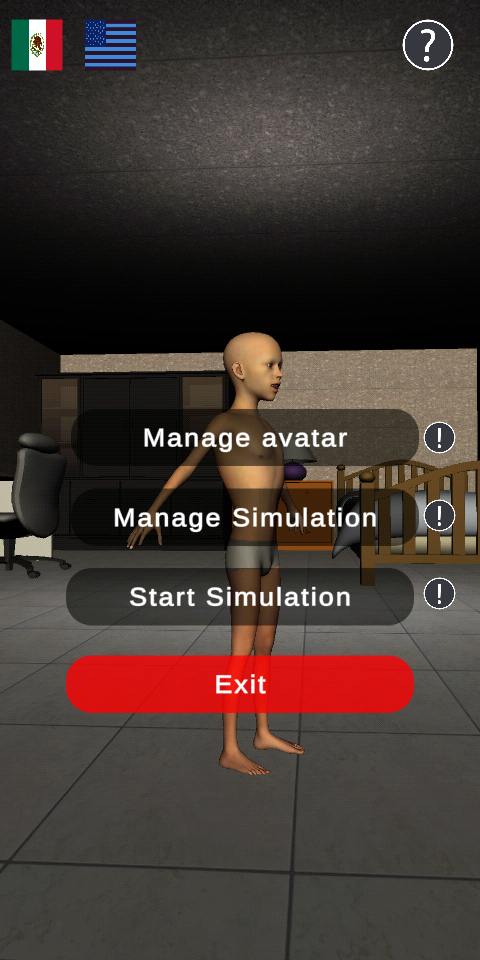
\includegraphics[width=0.18\textwidth]{Figs/Echartea1}&
         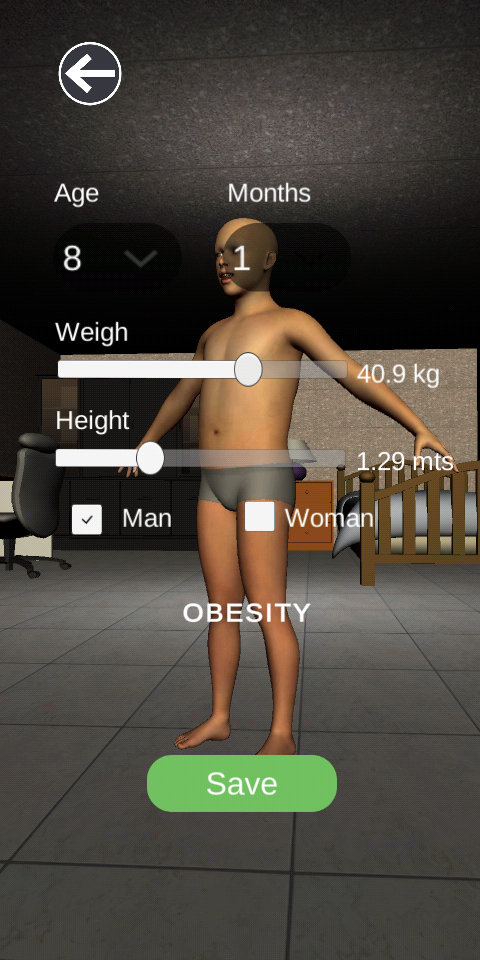
\includegraphics[width=0.18\textwidth]{Figs/Echartea2}&
         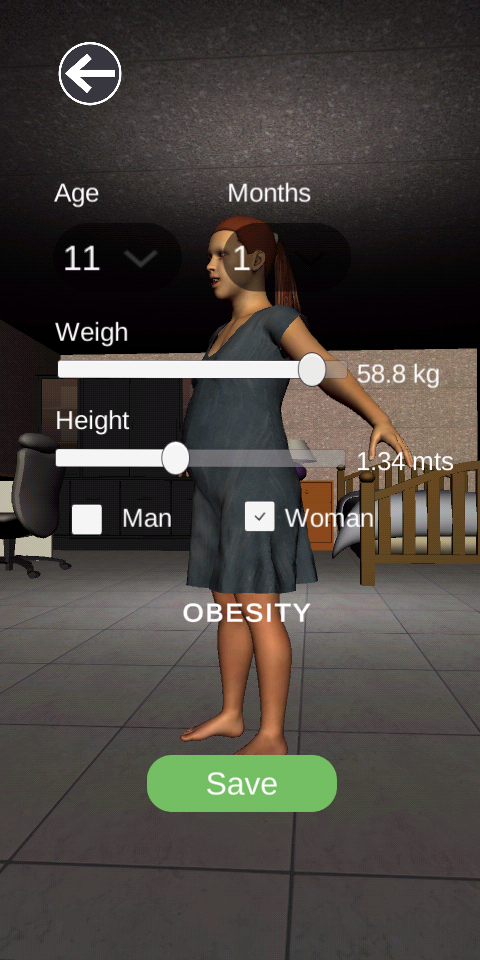
\includegraphics[width=0.18\textwidth]{Figs/Echartea3}\\
          \end{tabular}
\end{center}
\end{block} 
\end{frame}

\begin{frame}{\citetitle{Avatar3d_Echartea_2021} (3)}
\note[item]{When user presses the manage simulation button, a screen that allows the user to configure the meals, physical activity, BMI equation and simulation duration (in days or weeks) is shown }
\note[item]{When user presses the start simulation button, a screen that allows the user to start or stop the simulation is shown. }
\note[item]{When the simulation was started, two meal options are presented to the user, so the meal choose will affect the appeareance of the avatar along the simulation time}

\begin{block}{Screens of the proposed app (2)} 
\begin{center}
     \begin{tabular}{ccc}
         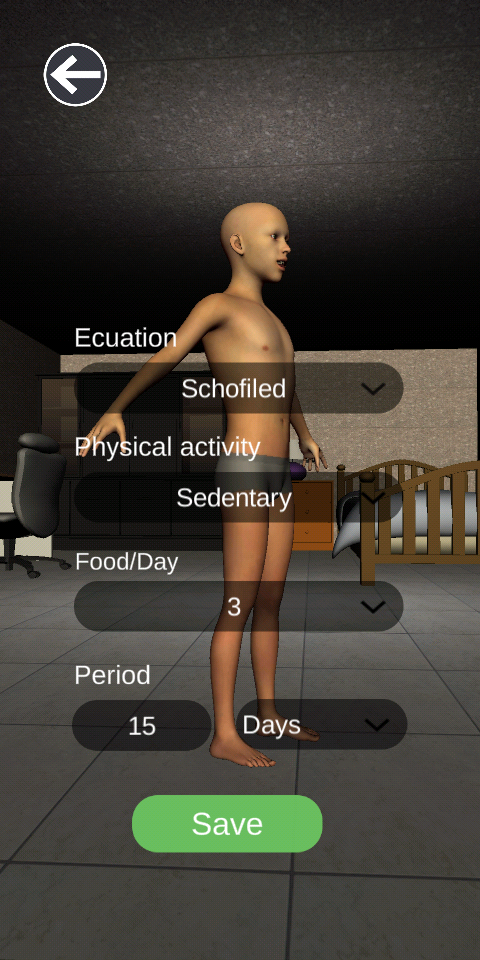
\includegraphics[width=0.18\textwidth]{Figs/Echartea4}&
         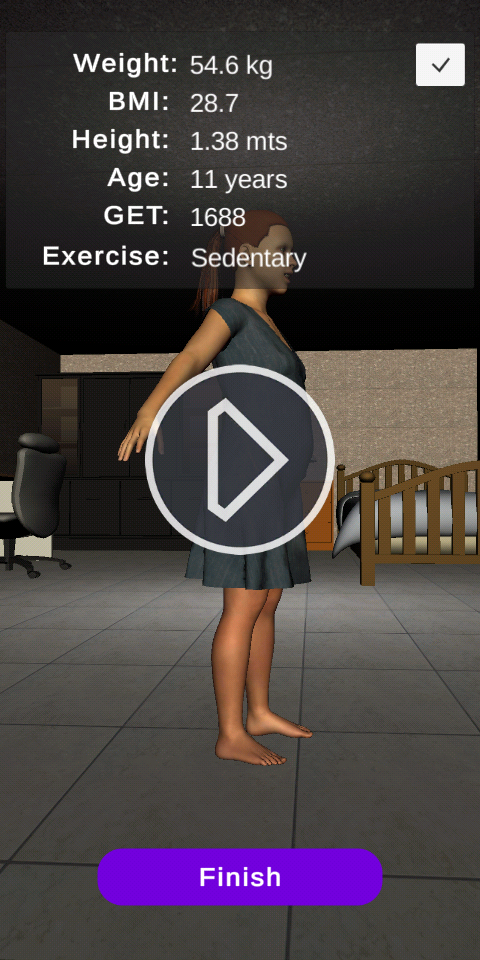
\includegraphics[width=0.18\textwidth]{Figs/Echartea5}&
         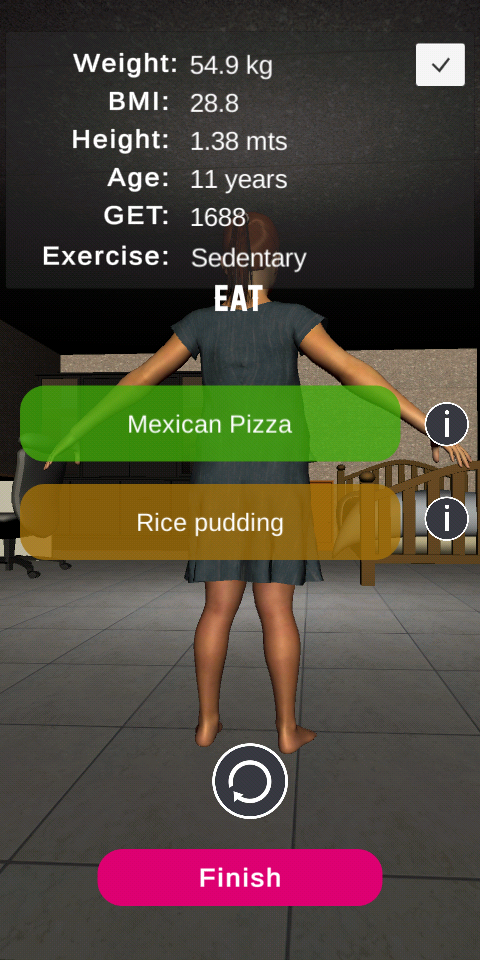
\includegraphics[width=0.18\textwidth]{Figs/Echartea6}\\
          \end{tabular}
\end{center}
\end{block} 
\end{frame}


\begin{frame}{\citetitle{Avatar3d_Echartea_2021} (4)}

\note[item]{For each food option, the user can show the nutritional information of that meal.}
\note[item]{When the simulation finishes, both initial and final avatars and the BMI are displayed. In this specific case, the weight difference is low so it is not possible to note the avatar's change.}
\note[item]{This project is almost finished since the graduate student is on the final test and evaluation of the app. We are going to report the results in a conference paper, and if possible, we are going to write a journal paper.}

\begin{block}{Screens of the proposed app (3)} 
\begin{center}
     \begin{tabular}{cc}
         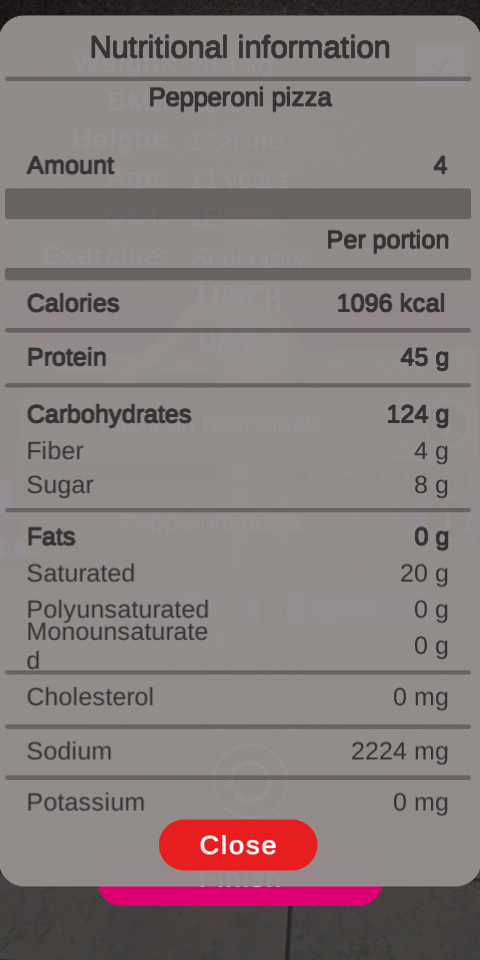
\includegraphics[width=0.18\textwidth]{Figs/Echartea9}&
         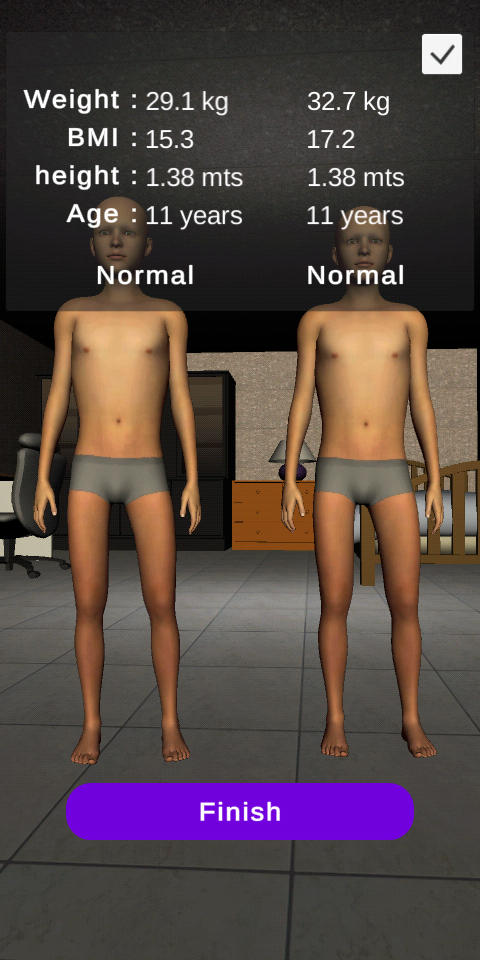
\includegraphics[width=0.18\textwidth]{Figs/Echartea8}\\

          \end{tabular}
\end{center}
\end{block} 
\end{frame}


